\documentclass[prd,preprintnumbers,floatfix,
nofootinbib,superscriptaddress]{revtex4}

%------------------

\usepackage{float}
\usepackage{nicefrac}
\usepackage{mathtools}
\usepackage{amsfonts}
\usepackage{amssymb}
\usepackage{amsmath}
\usepackage{graphicx}
\usepackage{subfigure}
\usepackage{array}
\usepackage{dcolumn}
\usepackage{bm}
\usepackage{esint}
\usepackage{xcolor}
\usepackage{longtable} % long tables
\usepackage{hyperref}
\usepackage{verbatim}
\usepackage{epsfig}
\usepackage{slashed}
\usepackage{color}


\newcommand{\diff}{\mathrm{d}}
\newcommand{\ket}[1]{\ensuremath{\left|#1\right\rangle}}
\newcommand{\bra}[1]{\ensuremath{\left\langle #1\right|}}
\newcommand{\TS}{\mathrm{TS}}
\newcommand{\LLH}{\mathrm{LLH}}
\newcommand{\M}{\mathcal{M}}
%
\newcommand{\I}{\ensuremath{I}}
\newcommand{\II}{\ensuremath{{I\!I}}}
\newcommand{\III}{\ensuremath{{I\!I\!I}}}
\newcommand{\IV}{\ensuremath{{I\!V}}}

\begin{document}
\title{Parity and signature test for the vector-vector system}

%%%%%%%%%%
\author{Mikhail Mikhasenko}
\email[e-mail: ]{mikhail.mikhasenko@cern.ch}
\affiliation{CERN-EP, CH-1211, Geneva, Switzerland}
%%%%%%%%%%

%%%%%%%%%%
\date{\today}
%%%%%%%%%%

%%%%%%%%%%
\begin{abstract}
  We present a construction of the reaction amplitude
  for inclusive production of the resonance decaying to a pair of identical vectors, as $J/\psi J/\psi$, $\phi\phi$, $Z^0 Z^0$.
  The method provides possibility to determine the spin and parity of the signal in the model-independent way.
  The test of the quantum-number hypotheses is demonstrated on the Standard Model decay of the Higgs particle to four leptons.
\end{abstract}
%%%%%%%%%%

\nopagebreak
\maketitle

\definecolor{cola}{rgb}{0.9,0.62,0.0}
\definecolor{colb}{rgb}{0.337, 0.706, 0.914 }
\definecolor{colc}{rgb}{0.0, 0.62, 0.451}
%
\section{Introduction}

% With the observation of the Higgs boson in 2013 the Standard Model was complete.
Formation of the hadronic matter is least understood part of the Standard Model.
Despite the fact that fundamental theory of strong interaction is known,
the theory degrees of freedom change at the low energy where hadronic phenomena emerges.
The constituent quark model successfully describes the majority of the observed hadronic states, however not all. Over the last decade we have witnessed overwhelming evidence of unexpected phenomena beyond the quark model that includes observation
of $XYZ$ states in the charminium spectrum~\cite{Godfrey:2008nc}, the pentaquark states~\cite{Aaij:2015tga,Aaij:2019vzc},
as well as resonance-like phenomena of hadronic rescattering singularizes~\cite{Alexeev:2020lvq}.

The observation of the threshold enhancement in the $J/\psi J/\psi$ spectrum~\cite{Aaij:2020xyz}
might lead to a new milestone in understanding of the hadron formation
through the mechanism for binding four charm quarks~\cite{Liu:2019zoy}.
The spin parity of the observed candidates is a critical part of the puzzle,
and moreover, as we present in the paper, it is accessible experimentally.

The signal in the pair of $J/\psi$ is not the only intriguing phenomena which is seen in the decay to two vectors.
The $\phi\phi$ pairs produced in central exclusive reactions hint a resonance signal, that is a candidate for a tensor glueball~\cite{Lebiedowicz:2019jru}.
The proposed approach sets the ground for the complete partial wave analysis of the high statistics $pp\to pp K^+K^-K^+K^-$ that
should be possible with the model LHC data.
One find the same signature of the Standard Model (SM) decay of the Higgs boson $H\to Z^0Z^0$.
% and possible Beyond Standard Model signal in $4l$ channel.
To conclude in favor of $0^+$ hypothesis for the spin-parity of the Higgs boson
several phenomenological models were compared on the combined dataset of several decay channels~\cite{Aad:2013xqa,CMS:2018mmw}.
% \cite{Bolognesi:2012mm,Gao:2010qx}
In contrast, we discuss the anatomy of the assumption-free approach.

The two key constraints that determine the properties of the decay are the parity conservation and the permutation symmetry.
One consequence of these constraints is known as the Landau-Yang theorem~\cite{Yang:1950rg,Landau:1948kw}.
The theorem states that a massive boson with $J^P = 1^+$ and all the natural quantum numbers and odd spin cannot decay into two on-shell photons.
The theorem follows naturally from the general equations we provide.
A parity-signature test of a signal in $\phi\phi$ system have been discussed in the past by several authors~\cite{Trueman:1978kh,Chang:1978jb,Collins:1977iv}.
Once we confirm the conclusion of Ref.~\ref{Trueman:1978kh} for the general vector-vector system, we test the modern statistical methods to separating spin hypothesis.

The paper is organized as follows. The reaction amplitude is presented in Sec.~\ref{sec:reaction.amplitude}.
In Sec.~\ref{sec:symmetries} we discuss the symmetry constraints.
We state the test statistics discriminator in Sec.~\ref{sec:test.statistics}.
The method is demonstrates on the SM Higgs decay in Sec.~\ref{sec:higgs}.

%                                      _|  _|    _|                      _|
%    _|_|_|  _|_|_|  _|_|    _|_|_|    _|      _|_|_|_|  _|    _|    _|_|_|    _|_|
%  _|    _|  _|    _|    _|  _|    _|  _|  _|    _|      _|    _|  _|    _|  _|_|_|_|
%  _|    _|  _|    _|    _|  _|    _|  _|  _|    _|      _|    _|  _|    _|  _|
%    _|_|_|  _|    _|    _|  _|_|_|    _|  _|      _|_|    _|_|_|    _|_|_|    _|_|_|
%                            _|
%                            _|

\section{Angular amplitude} \label{sec:reaction.amplitude}
We focus on an inclusive production process $p p'\to X$.
Despite the vectors are identical, it is convenient to distinguish them in the
reaction amplitude calling them $V_1$ and $V_2$. In that way, we can make sure that the amplitude
is symmetric on permutation of indices $1$ and $2$.

A negligibly small polarization was measured in the prompt production of charmonium~\cite{Aaij:2013nlm,Chatrchyan:2012woa,CDF:2011ag, Aaij:2013oxa,Sirunyan:2018bfd}.
However, for the peripheral processes, e.g. central exclusive production (CEP) a significant polarization is expected~\cite{Pasechnik:2010pq}.
Therefore, we consider a general case of arbitrary polarization.
For numerical tests however, we restrict ourselves to the unpolarized case.

The production frame is set up in the rest frame of $X$ as a plane that contains three-vectors of the
production reaction, i.e. $\vec p$, and $\vec p'$. The normal to the plane gives $y$ axis (precisely $\vec p\,'\times \vec p$) as shown in Fig.~\ref{fig:production}.
We use the Gottfried-Jackson (GJ) frame for defining in the $x$ and $z$ axis in the production plane~\cite{Gottfried:1964nx}.
We note, however, that the choice of $x$ and $z$ axes is not unique, two other two common definition of the production frame are the helicity (HX) frame
defined by the direction of motion of $X$ itself in the lab frame, and the Collins-Soper (CS) frame where $z$ is defined by bisection of the angle between $\vec p$ and $\vec p\,'$~\cite{Faccioli:2010kd}.
\begin{figure}
  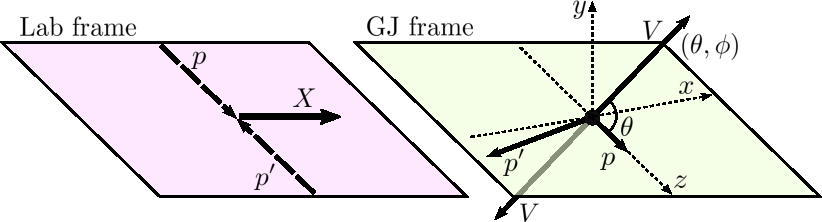
\includegraphics[width=0.6\textwidth]{../plots/production_GJ.pdf}
  \caption{Schematic view of production kinematics of $X$ state at the $pp$ collider.
  The Gottfried-Jackson frame is used for describing production kinematics.
  It is defined in the rest frame of $X$ by the vectors of the beam particles:
  $\vec z = \vec p / |\vec p|$, $\vec y = \vec p' \times \vec p / |\vec p' \times \vec p|$, $\vec x = \vec y \times \vec z$.
  The spherical angles $(\theta,\phi)$ are the angles of one of two decay vectors in the GJ frame.
  The black arrows shows three dimensional vectors of particles.
  The three-momenta of the produced vectors are $\vec p_{V_1}$ and $\vec p_{V_2}$.
  }
  \label{fig:production}
\end{figure}

The full kinematics of the decay is described by 6 angles: a pair of sperical angles $(\theta,\phi)$ of the momentum of $V_1$ in the GJ frame, and two pairs of the spherical angles $(\theta_i,\phi_i)$, $i=1,2$
for decay of the vectors in their own helicity frames.
We note that the angles $\phi_i$ can also be defined in the $X$ rest frame as shown in Fig.~\ref{fig:decay}
since they do not effected by the boosts.

The spin of the decay particle defines rotational properties of the system of the decay products~\cite{DPD}.
Every configuration of the three-momenta of the final state particles in the $X$ rest frame
can be considered as a solid body for which the orientation is described by three angles:
the pair of spherical angles $(\theta,\phi)$ describe the direction of $\vec p_{V_1}$,
the third angle $\phi_1$ is the azimuthal direction of $\mu^+$ in the $V_1$ rest frame (see Fig.~\ref{fig:production} and Fig.~\ref{fig:decay}).
% The intensity of the decay is defined as a differential cross section over angular variables,
% $I = \diff \sigma / \diff \Omega\,\diff \Omega_1\,\diff \Omega_2$, where
% $\diff\Omega = \diff\cos\theta \diff \phi$; the $\Omega_i$, $i=1,2$ are the spherical angles of the decay products of the two vector particles in the corresponding helicity frames as shown in Fig.~\ref{fig:X.decay}.
%
% The intensity reads:
\begin{align}
    I(\Omega,\Omega_1,\Omega_2) &= (2J+1) \sum_{M,M'}R_{M,M'}\,
    D_{M,\nu}^{J}(\phi,\theta,\phi_1) D_{M',\nu'}^{J*}(\phi,\theta,\phi_1)
    \sum_{\xi_1,\xi_2}^{\{-1,1\}}
    A^{\nu}_{\xi_1,\xi_2}(\Omega_1,\Omega_2) A^{\nu'*}_{\xi_1,\xi_2}(\Omega_1,\Omega_2),
\end{align}
where we have explicitly separated the production and decay part of the amplitude.
The production dynamics encapsulated into the polarization matrix $R_{M,M'}$.
The decay amplitude $X\to V(\mu^+\mu^-)V(\mu^+\mu^-)$ is denoted $A^{\lambda}_{\xi_1,\xi_2}$
with $\nu$ being the difference of the vector's helicities, and $\xi$ being the difference of the muon's helicities. $J$ and $M$ are the spin and spin projection of the $X$.
The decay amplitude is described by the remaining three angles: $\theta_1$, $\theta_2$, and $\Delta\phi = \phi_2-\phi_1$.
% ,$I_0$ is the total integrated intensity
% We used the angle $\phi_1$ as the third Euler angle for the orientation of
% the solid body of the decay products vectors~\cite{DPD}. With this choice the
% decay amplitude is determined by just three angles:
% the polar angles of the vector decay, and the azimuthal difference of the decay planes (see Fig.~\ref{fig:X.decay})
\begin{align}
  A^{\nu}_{\xi_1,\xi_2}(\theta_1,\theta_2,\Delta\phi) &= 3
  \sum_{\lambda_1,\lambda_2}
  \delta_{\nu,\lambda_1-\lambda_2} (-1)^{1-\lambda_2}
  H_{\lambda_1\lambda_2}
  d_{\lambda_1,\xi_1}^{1}(\theta_1) d_{\lambda_2,\xi_2}^{1}(\theta_2).
  e^{i\lambda_2 \Delta\phi}
\end{align}
The factor $(-1)^{1-\lambda_2}$ is related to the Jacob-Wick particle-2 phase convention~\cite{Jacob:1959at}.
Once the phase is factored out of the helicity coupling matrix $H_{\lambda_1,\lambda_2}$
the symmetry relations for $H$ are significantly simpler.
\begin{figure}
  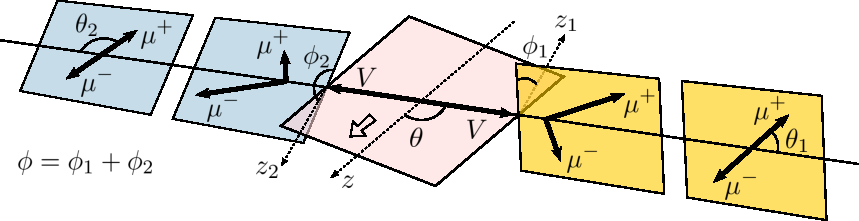
\includegraphics[width=0.8\textwidth]{../plots/angles.pdf}
  \caption{Schematic view of the $X\to V(\mu^+\mu^-)\,V(\mu^+\mu^-)$ decay kinematics.
  The central three planes show orientation of vectors in the $X$ rest frame.
  The right and left most planes show the decay angles of $J/\psi_1$ and $J/\psi_2$ in the rest frame, respectively.
  % The black arrows shows three dimensional vectors of particles.
  % A shaped arrow gives the direction of polarization of $X$.
  }
  \label{fig:decay}
\end{figure}


% \begin{equation} \label{eq:delta}
%   \sum_M d_{M,\lambda_1-\lambda_2}^{J}(\theta) d_{M,\lambda_1'-\lambda_2'}^{J}(\theta) = \delta_{\lambda_1-\lambda_2,\lambda_1'-\lambda_2'}.
% \end{equation}
% On contrast, the observed non-trivial dependence of the intensity on $\cos\theta$
% would indicate polarization of the initial state.
% Once the orientation of the production plane is averaged, the intensity becomes a function of just three quantities: polar decay angles of leptons, the difference on the azimuthal angles, $\Delta\phi = \phi_1+\phi_2$. It is easy to see transforming the azimuthal dependence,
% \begin{equation}
% i\lambda_1\phi_1+i\lambda_2\phi_2 = i(\lambda_1-\lambda_2)\phi_1+i\lambda_2\Delta\phi
% \end{equation}
% The first term on the left side of the expression vanishes once the amplitude is multiplied
% to the conjugated with help of Eq.~\eqref{eq:delta}.

%
%                                                                  _|
%    _|_|_|  _|    _|  _|_|_|  _|_|    _|_|_|  _|_|      _|_|    _|_|_|_|  _|  _|_|  _|    _|
%  _|_|      _|    _|  _|    _|    _|  _|    _|    _|  _|_|_|_|    _|      _|_|      _|    _|
%      _|_|  _|    _|  _|    _|    _|  _|    _|    _|  _|          _|      _|        _|    _|
%  _|_|_|      _|_|_|  _|    _|    _|  _|    _|    _|    _|_|_|      _|_|  _|          _|_|_|
%                  _|                                                                      _|
%              _|_|                                                                    _|_|


\section{Symmetry constraints} \label{sec:symmetries}
The matrix of the helicity couplings is strictly defined by
 % $H_{\lambda_1,\lambda_2}$ is a $3\times 3$ matrix
\begin{equation} \label{eq:helicity.def}
  H_{\lambda_1,\lambda_2} = \bra{JM;\lambda_1,\lambda_2}\hat{T}\ket{JM},
\end{equation}
where the bra-state is the protected two-particle state in the particle-2 convention,
the ket-state is the decaying state with the defined spin $J$ and the spin projection to the $z$ axis in the GJ frame, $M$~\cite{Martin.Spearman}.
The matrix is constrained by parity and permutation symmetry.
The parity relates the opposite values of the vector's helicities:
\begin{equation} \label{eq:parity}
H_{\lambda_1,\lambda_2} = P (-1)^J H_{-\lambda_1,-\lambda_2},
\end{equation}
with $P$ being the internal parity of the decaying particle.
Identity of the decay particle relates the helicity matrix with the transposed one.
\begin{equation} \label{eq:permutation}
H_{\lambda_1,\lambda_2} = (-1)^J H_{\lambda_2,\lambda_1},
\end{equation}
The matrices of the helicity couplings are symmetric (anti-symmetric) for the even-spin (odd-spin) decay particle.
Combining two symmetries we split all possible quantum numbers $J^P$ into four groups as shown in Tab.~\ref{tab:couplings}.
\begin{table}
  \caption{Possible quantum numbers of the decaying particle $X$ separated to four groups with respect of symmetry of the helicity matrix. The framed quantum numbers in the last column have additional restrictions due to the maximal value of the spin projection.}
  \label{tab:couplings}
  \begin{ruledtabular}
  \begin{tabular}{c | r | r | l}
    group & $(-1)^{J}$ & $P(-1)^{J}$ & explicit $J^P$\\\hline
    \I    & even($+$) &   natural($+$) & \fbox{$0^+$}, $2^+$, $4^+$, $6^+$\\
    \II   & even($+$) & unnatural($-$) & \fbox{$0^-$}, $2^-$, $4^-$, $6^-$\\
    \III  & odd($-$)  &   natural($+$) &        $1^-$, $3^-$, $5^-$, $7^-$\\
    \IV   & odd($-$)  & unnatural($-$) & \fbox{$1^+$}, $3^+$, $5^+$, $7^+$
  \end{tabular}
  \end{ruledtabular}
\end{table}
The relations Eq.~\eqref{eq:parity} and Eq.~\eqref{eq:permutation} greatly reduce the number of free components of the helicity matrix.
\begin{align}
  H_\I&=\begin{pmatrix}
    b & a & c\\
    a & d & a\\
    c & a & b
  \end{pmatrix}_S&
  H_\II&=\begin{pmatrix}
    b & a &  \\
    a &   & -a\\
      & -a & -b
  \end{pmatrix}_S&
  H_{\III}&=\begin{pmatrix}
      & a &  \\
    -a &   & -a\\
      & a &
  \end{pmatrix}_A&
  H_{\IV}&=\begin{pmatrix}
      & a & c\\
    -a &   & a\\
    -c & -a &
  \end{pmatrix}_A
\end{align}
There are three special cases, $0^+$ of the first group for which $a=c=0$,
$0^-$ in the second group with $a=0$, and $1^+$ in the forth group with $c=0$.
% \begin{align} \label{eq:matrices.spec}
%   H_\I^{(0^+)}&=\begin{pmatrix}
%     b & & \\
%     & d &\\
%     & & b
%   \end{pmatrix}_S&
%   H_\II^{(0^-)}&=\begin{pmatrix}
%     b &  &  \\
%      &   & \\
%       &  & -b
%   \end{pmatrix}_S&
%   H_{\IV}^{(1^+)}&=\begin{pmatrix}
%       & a & \\
%     -a &   & a\\
%       & -a &
%   \end{pmatrix}_A
% \end{align}

%
%    _|                            _|
%  _|_|_|_|    _|_|      _|_|_|  _|_|_|_|
%    _|      _|_|_|_|  _|_|        _|
%    _|      _|            _|_|    _|
%      _|_|    _|_|_|  _|_|_|        _|_|


\section{Testing hypothesis} \label{sec:test.statistics}
% \section{Test statistics}
The most powerful method for testing spin hypothesis is the multidimensional fit.
For simplicity we consider the case of the negligible polarization in three dimensions, while all discussion is easy to generalize to the five dimensional case that includes
the polarization degrees of freedom.
The test statistics is defined by
\begin{align}
  \TS_{M/M'} = \LLH_M - \LLH_{M'},
\end{align},
where the $\LLH_M$ is the maximized value of the log likelihood over the set of helicity couplings.
\begin{equation}
  \LLH_M = \frac{1}{N_\mathrm{ev}} \sum_{e=1}^{N_\mathrm{ev}} \log I(\tau_e|M\{\hat{h}\}).
\end{equation}
The intensity $I(\tau_e|\hat{c})$ is calculated for the kinematic variables of the event $e$.
The optimized model parameters are demoted by $\hat{h}$. We use a convenient normalization condition $\mathrm{Tr}(HH^\dagger) = \mathbb{I}$.
% Normalization for the fitted density is established using the relation,
% \begin{align}
%   \int I(\theta_1,\theta_2,\Delta\phi)\,\frac{\diff\cos\theta_1\,\diff\cos\theta_2\,\diff \Delta\phi}{8\pi} = N \sum_{\lambda_1,\lambda_2} |H_{\lambda_1\lambda_2}|^2.
% \end{align}
% Fig.~\ref{fig:TS.fixedH} shows an example of the test-statistics distribution obtained on the statistical sample of the fixed group-\III coupling matrix.

%
%            _|        _|
%  _|_|_|    _|_|_|
%  _|    _|  _|    _|  _|
%  _|    _|  _|    _|  _|
%  _|_|_|    _|    _|  _|
%  _|
%  _|

Distribution over $\Delta\phi$ angle once $\theta_1$ are $\theta_2$ are integrated:
\begin{align}
  \frac{2\pi}{N}\frac{\diff N}{\diff \Delta\phi} = 1
   + \frac{h_{1,1} h_{-1,-1}^*}{2} \cos(2 \Delta\phi),
\end{align}
The sign of the $\cos(2\Delta\phi)$ component depends on $J^P$: it is positive for quantum numbers of the first group, and negative for the ones in the second group.
The decays from the third and fourth groups do not show $2\Delta\phi$ dependence.
This sign can be determined by either fitting $\Delta\phi$ spectra, or calculating $\cos(2\Delta\phi)$ moment,
\begin{equation}
  M_{\cos(2\Delta\phi)} = \frac{1}{N_D}\sum_{e=1}^{N_D} \cos(2\Delta\phi_e).
\end{equation}

Useful relations for $\cos\theta$ integrals
\begin{align}
  3 \sum_{\xi}^{\{-1,1\}} \int_{-1}^{1} \diff \cos\theta\, d_{\lambda,\xi}^{1}(\theta) d_{\lambda',\xi}^{1}(\theta) =
  \begin{pmatrix}2 & 0 & 1\\0 & 2 & 0\\1 & 0 & 2\end{pmatrix}_{\lambda\lambda'},\\
  %
  % 3 \sum_{\xi}^{\{-1,1\}} \int_{0}^{1} \diff \cos\,\theta d_{\lambda,\xi}^{1}(\theta) d_{\lambda',\xi}^{1}(\theta) =
  % \frac{1}{2}\begin{pmatrix}2 & -\frac{1}{\sqrt{2}} & 1\\-\frac{1}{\sqrt{2}} & 2 & \frac{1}{\sqrt{2}}\\1 & \frac{1}{\sqrt{2}} & 2\end{pmatrix}_{\lambda\lambda'},\\
  %
\end{align}


%
%  _|        _|
%  _|_|_|          _|_|_|    _|_|_|    _|_|_|
%  _|    _|  _|  _|    _|  _|    _|  _|_|
%  _|    _|  _|  _|    _|  _|    _|      _|_|
%  _|    _|  _|    _|_|_|    _|_|_|  _|_|_|
%                      _|        _|
%                  _|_|      _|_|


\section{Testing the SM Higgs decay} \label{sec:higgs}
To demonstrate the method
The most famous particle decaying to two identical vectors is the Higgs boson.
In order to validate out approach we performed analysis of the reaction $H\to Z(\mu^+\mu^-)Z(\mu^+\mu^-)$.
% A sample of $500$ events was generated using the MadGraph.
The interaction vertex of Higgs with a pair of $Z^0$ bosons is $2i m_Z^2/v\,g^{\mu\nu}$,
hence the helicity amplitude reads:
\begin{equation} \label{eq:HZZ}
  A^{H\to ZZ}_{\lambda_1,\lambda_2} = 2i\frac{m_Z^2}{v} (\epsilon_1^*(\lambda_1)\cdot\epsilon_2^*(\lambda_2)).
\end{equation}
Using the explicit expressions for the polarization $\epsilon$ vectors,
we find a special case of the matrix for group-$\I$,
\begin{equation}
  H^{H\to ZZ} = \frac{\mathbb{I}}{\sqrt{3}} + O(p^2)
\end{equation}
The matrix is proportional to identity (S-wave) close to the nominal $ZZ$ production threshold,
the contribution of the $D$-wave is suppressed by $|\vec p\,|^2/m_Z^2$.

\begin{figure}
  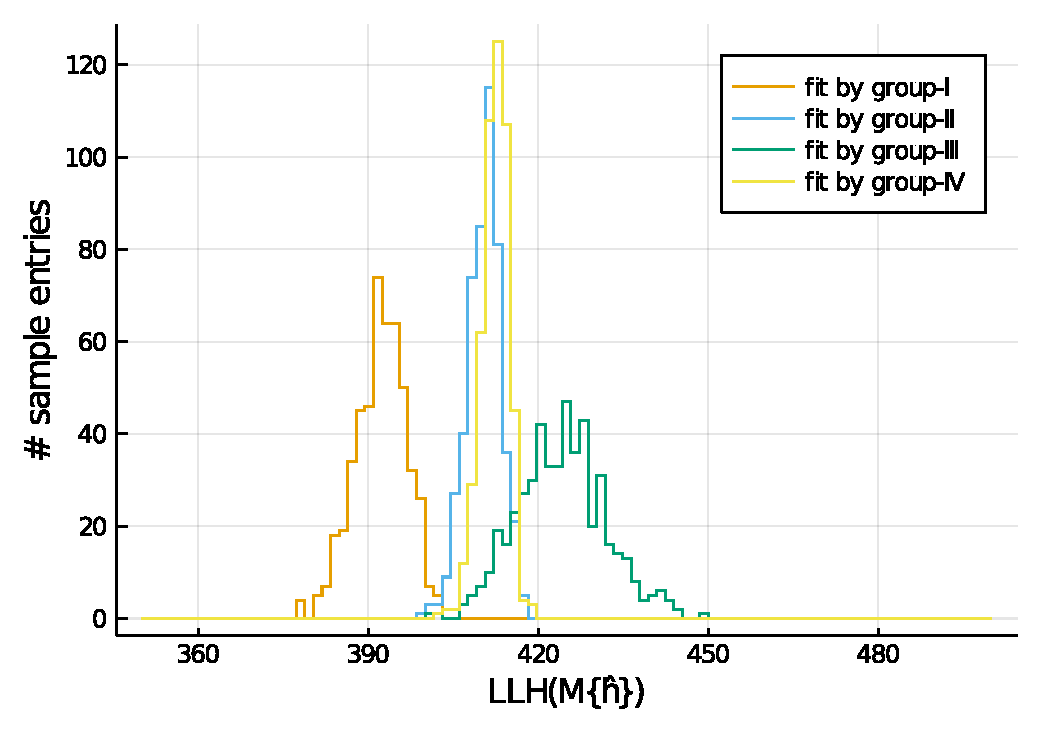
\includegraphics[width=0.48\textwidth]{../plots/llh_testing_higgs.pdf}
  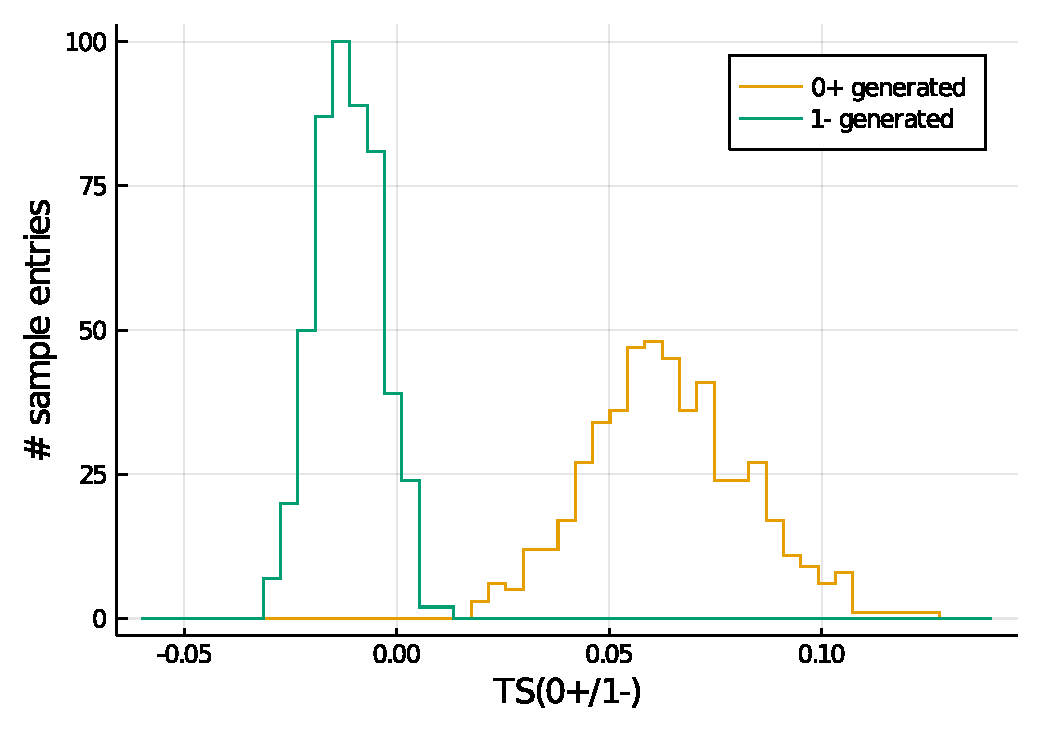
\includegraphics[width=0.48\textwidth]{../plots/TS_0p_vs_1m.pdf}
  \caption{Test statistics distribution testing hypothesis of groups $\I-\IV$ and the special cases on the statistical ensemble of the $500$ events data samples generated based on
  the fixed group-$\III$ coupling matrix. }
  \label{fig:TS.fixedH}
\end{figure}

\begin{figure}
  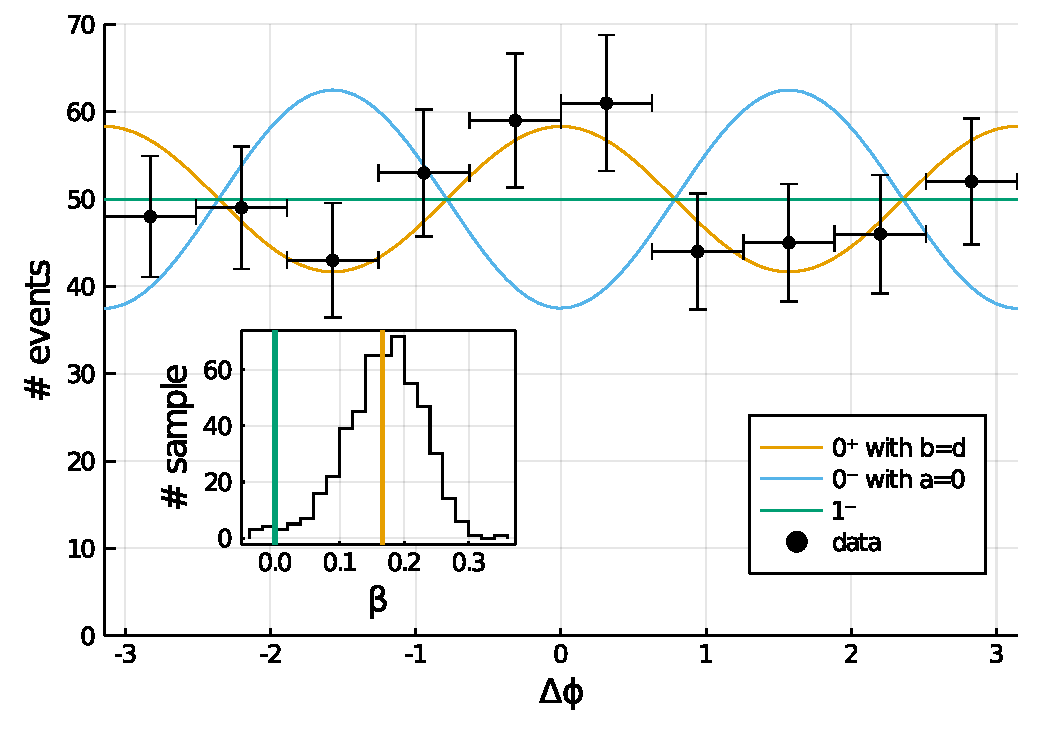
\includegraphics[width=0.48\textwidth]{../plots/phi_higgs.pdf}
  \caption{}
  \label{fig:higgs.phi}
\end{figure}

\section{Conclusion}


\section*{Acknowledgement}
The project was motivated by a discussion in the LHCb Amplitude Analysis group.
We thank Biplab Day for organizing seminar dedicated to $X\to VV$.
We would like to gratefully thank Alessandro Pilloni for useful comments on the work.
We thank Liupan An and Ronan McNulty for finding practical cases for the analysis.

\appendix

\section{Corrections for $X\to V(K^+K^-)V(K^+K^-)$}
\begin{align}
  3 \int_{-1}^{1} \diff \cos\,\theta d_{\lambda,0}^{1}(\theta) d_{\lambda',0}^{1}(\theta) =
  \begin{pmatrix}1 & 0 & -1\\0 & 1 & 0\\-1 & 0 & 1\end{pmatrix}_{\lambda\lambda'}.
\end{align}

\section{Polarization vectors}

For calculation of the Higgs decay ampluitude in Eq.~\eqref{eq:HZZ}
we used explicit expressions for the polarization vectors:
\begin{align}
  \epsilon_z^{\mu}(\pm1) &= \frac{1}{\sqrt{2}} \left( 0,\mp 1,-i,0 \right), &
  \epsilon_z^{\mu}(0) &= \frac{1}{m_Z} \left(p,0,0,E\right),
\end{align}
where $E$, $p$, and $m_Z$ are the energy, momentum, and the mass of the $Z$ boson.
The general expressions for the rotational vectors follows:
\begin{align}
  % \epsilon_1(\pm1) &= R_z(\Delta\phi) R_y(\theta) (0,-i,\mp 1,0)\frac{1}{\sqrt{2}},\\
  % \epsilon_2(\pm1) &= R_z(\Delta\phi) R_y(\theta) R_y(\pi) (0,-i,\mp 1,0)\frac{1}{\sqrt{2}};\\
  % \epsilon_1(0) &= R_z(\Delta\phi) R_y(\theta) (-p,0,0,E)\frac{1}{m},\\
  % \epsilon_2(0) &= (-1) R_z(\Delta\phi) R_y(\theta) R_y(\pi) (-p,0,0,E)\frac{1}{m},
  \epsilon_1(\lambda) &= R_z(\phi) R_y(\theta) \epsilon_z(\lambda),\\
  \epsilon_2(\lambda) &= (-1)^{1-\lambda} R_z(\phi) R_y(\theta) R_y(\pi) \epsilon_z(\lambda),\\
\end{align}
where $R_y(\phi)R_y(\theta)$ is a product of the three-dimensional rotation matrices
that transforms the vector $(0,0,1)$ to the direction $(\sin\theta\cos\phi,\,\sin\theta\sin\phi,\,\cos\theta)$.
The particle-2 requires additional rotation by $\pi$ about the $y$ axis. We also use the particle-two phase convention,
$(-1)^{1-\lambda_2}$ that adds an extra sign to the vector $\epsilon_2(0)$.

\section{$\eta s$ invariance}

\begin{equation}
  H = \begin{pmatrix}
    0 &1 &0 \\
    s & 0 &s\eta \\
    0 &\eta &0
  \end{pmatrix}
\end{equation}
The intensity reads:
\begin{align}
  I(H) &= \frac{s^{2} \eta^{2} \sin^{2}{\left (\theta_{1} \right )} \cos^{2}{\left (\theta_{2} \right )}}{2} + \frac{s^{2} \eta^{2} \sin^{2}{\left (\theta_{1} \right )}}{2} + \frac{s^{2} \sin^{2}{\left (\theta_{1} \right )} \cos^{2}{\left (\theta_{2} \right )}}{2} + \frac{s^{2} \sin^{2}{\left (\theta_{1} \right )}}{2} \\ \nonumber
   &\quad + \frac{s \eta \left(\cos{\left (- 2 \theta_{1} + 2 \theta_{2} + \Delta\phi \right )} + \cos{\left (2 \theta_{1} - 2 \theta_{2} + \Delta\phi \right )} - \cos{\left (2 \theta_{1} + 2 \theta_{2} - \Delta\phi \right )} - \cos{\left (2 \theta_{1} + 2 \theta_{2} + \Delta\phi \right )}\right)}{8}\\ \nonumber
   &\quad+\frac{\eta^{2} \sin^{2}{\left (\theta_{2} \right )} \cos^{2}{\left (\theta_{1} \right )}}{2} + \frac{\eta^{2} \sin^{2}{\left (\theta_{2} \right )}}{2} + \frac{\sin^{2}{\left (\theta_{2} \right )} \cos^{2}{\left (\theta_{1} \right )}}{2} + \frac{\sin^{2}{\left (\theta_{2} \right )}}{2}
\end{align}
The expression does not change under flip of $\eta$ and $s$ sign simultaneously.
Hence the group-$\III$ cannot be distinguished from the group-$\II$.

\bibliography{ref}
\end{document}




% \begin{align}
%   \frac{\diff^2 N}{\diff \cos\theta_1\,\diff \cos\theta_2} =
%   |H_{\lambda_1\lambda_2}|^2
%   \sum_{\xi_1,\xi_2}^{\{-1,1\}}
%   9|d_{\lambda_1,\xi_1}^{1}(\theta_1) d_{\lambda_2,\xi_2}^{1}(\theta_2)|^2.
% \end{align}

% \section{LS couplings}
%
% \begin{align}
%   H_{\lambda_1,\lambda_2} = (-1)^{j_2-\lambda_2} \sum_{ls} \sqrt{\frac{2l+1}{2j+1}}
%   \left\langle 1,\lambda_1;1,\lambda_2|s,\lambda_1-\lambda_2 \right\rangle
%   \left\langle L,0;s,\lambda_1-\lambda_2|j,\lambda_1-\lambda_2 \right\rangle H_{ls}.
% \end{align}
%
% \begin{align*}
%   1^-\otimes 1^-: && S:\qquad & {\color{cola} 0^+}\quad {\color{colb} 1^+}\quad {\color{colc} 2^+},\\
%                   && P:\qquad & \color{gray} 1^-\quad (0^-,1^-,2^-)\quad (1^-,2^-,3^-),\\
%                   && D:\qquad & {\color{colc} 2^+}\quad ({\color{colb} 1^+},{\color{colc} 2^+},3^+)\quad ({\color{cola} 0^+},{\color{colb} 1^+},{\color{colc} 2^+},3^+,4^+),\\
%                   && F:\qquad & \color{gray} 3^-\quad (2^-,3^-,4^-)\quad (0^-,1^-,2^-,3^-,4^-),\\
%                   && H:\qquad & 4^+\quad (3^+,4^+,5^+)\quad ({\color{colc} 2^+},3^+,4^+,5^+,6^+).
% \end{align*}

% \section{Odd and even spins}

% \begin{figure}
%   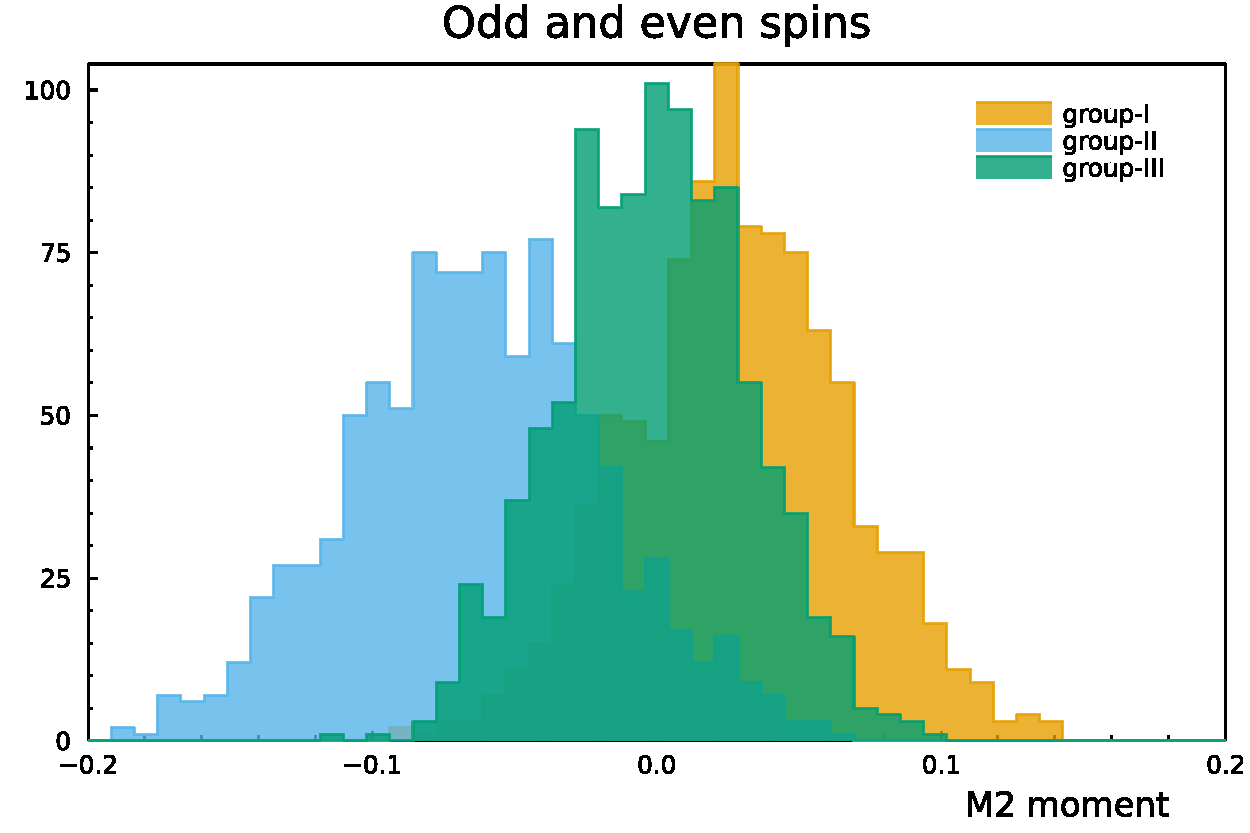
\includegraphics[width=0.46\textwidth]{../plots/moment_M2phi_Nev=500.pdf}
%   \caption{Distribution of $M_{\cos(2\Delta\phi)}$ for a sample of random coupling constants.
%   A sample of $500$ events is generated for every hypothesis of couplings.}
%   \label{}
% \end{figure}
%
% \begin{figure}
%   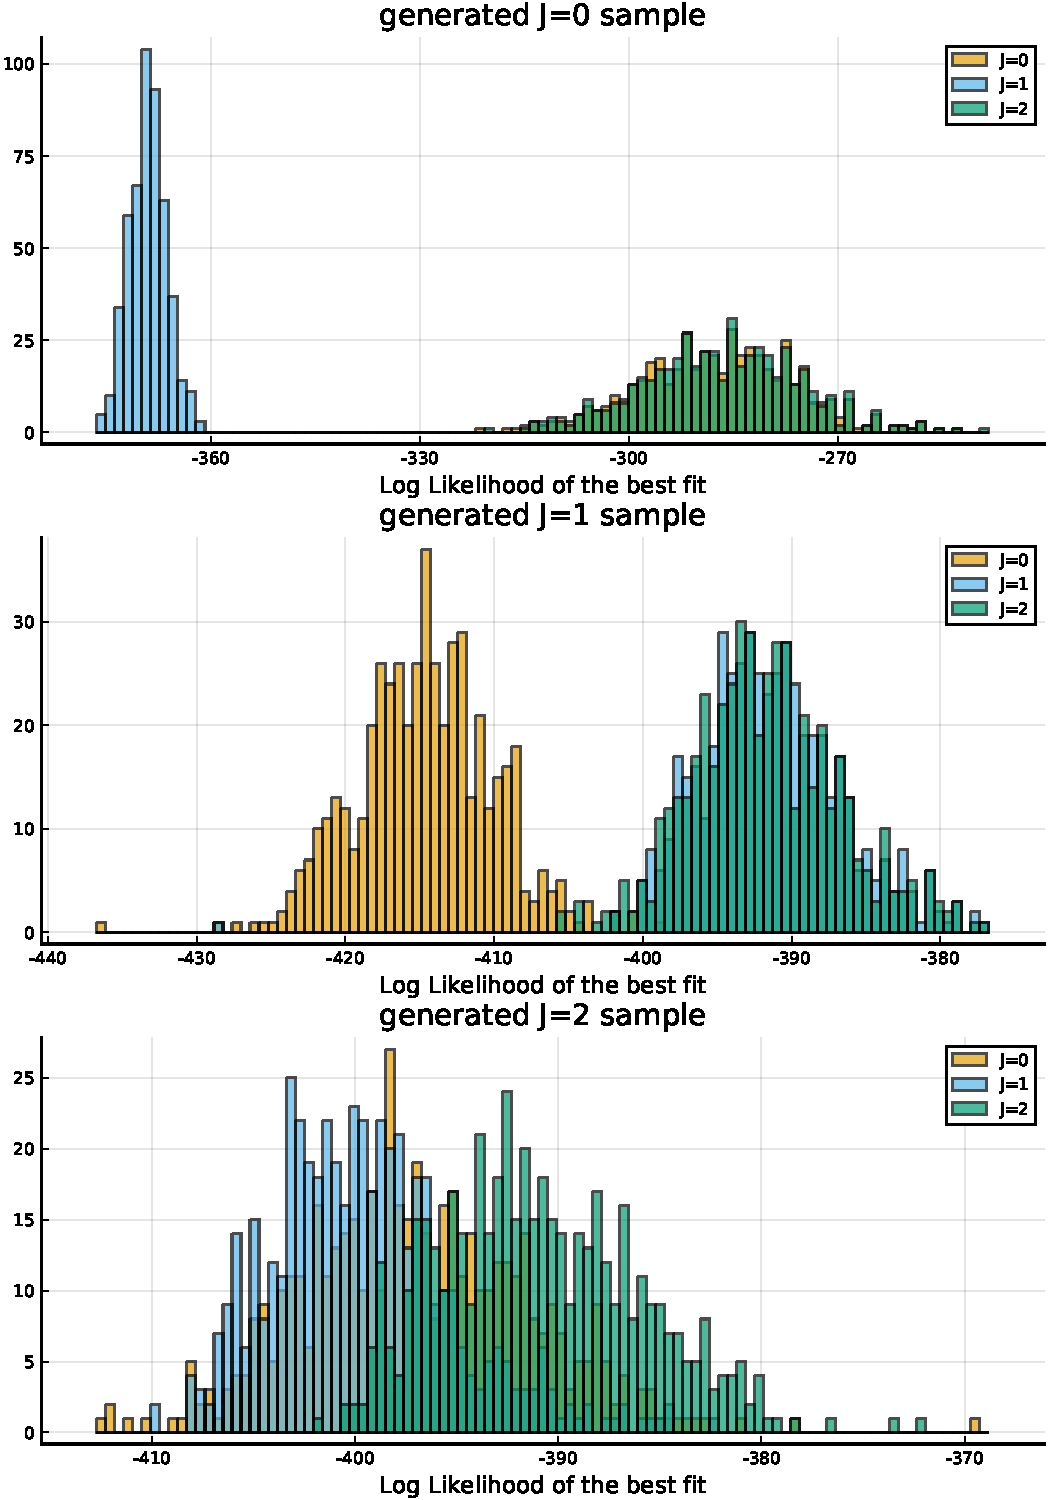
\includegraphics[width=0.9\textwidth]{../plots/llh_of_fit_of_J012.pdf}
%   \caption{Hypothesis testing with $500$ events}
%   \label{fig.3dfit}
% \end{figure}


% Matrices of couplings without the phase $(-1)^{j_2-\lambda_2}$ are symmetric (round brackets) or asymmetric (square parentheses)
% \begin{itemize}
%   \item $j = 0$:
% \begin{align*}
%   % l = 0, s = 0
%   \frac{\sqrt{3}}{3}
%   \begin{pmatrix}1 & 0 & 0\\0 & -1 & 0\\0 & 0 & 1\end{pmatrix}&&
%   % l = 2, s = 2
%   \frac{\sqrt{6}}{6}
%   \begin{pmatrix}1 & 0 & 0\\0 & 2 & 0\\0 & 0 & 1\end{pmatrix}
% \end{align*}
%   \item $j = 1$:
% \begin{align*}
%   % l = 0, s = 1
%   \frac{\sqrt{6}}{6}
%   \begin{pmatrix}-1 & -1 & 0\\-1 & 0 & 1\\0 & 1 & 1\end{pmatrix}&&
%   % l = 2, s = 1
%   \frac{\sqrt{3}}{6}
%   \begin{pmatrix}2 & -1 & 0\\-1 & 0 & 1\\0 & 1 & -2\end{pmatrix}&&
%   % l = 2, s = 2
%   \frac{1}{2}
%   \left[\begin{matrix}0 & -1 & 0\\1 & 0 & -1\\0 & 1 & 0\end{matrix}\right]
% \end{align*}
% \item $j = 2$:
% \begin{align*}
%   % l = 0, s = 2
%   \frac{\sqrt{30}}{30}
%   \begin{pmatrix}1 & \sqrt{3} & \sqrt{6}\\\sqrt{3} & 2 & \sqrt{3}\\\sqrt{6} & \sqrt{3} & 1\end{pmatrix}&&
%   % l = 2, s = 0
%   \frac{\sqrt{3}}{3}
%   \begin{pmatrix}1 & 0 & 0\\0 & -1 & 0\\0 & 0 & 1\end{pmatrix}&&
%   % l = 2, s = 1
%   \frac{1}{2}
%   \left[\begin{matrix}0 & -1 & 0\\1 & 0 & 1\\0 & -1 & 0\end{matrix}\right]&&
%   % l = 2, s = 2
%   \frac{\sqrt{7}}{14}
%   \begin{pmatrix}- \frac{2 \sqrt{3}}{3} & -1 & 2 \sqrt{2}\\-1 & -\frac{4 \sqrt{3}}{3} & -1\\2 \sqrt{2} & -1 & - \frac{2 \sqrt{3}}{3}\end{pmatrix}&&
%   % l = 4, s = 2
%   \frac{\sqrt{70}}{70}
%   \begin{pmatrix}\sqrt{6} & -2 \sqrt{2} & 1\\- 2 \sqrt{2} & 2\sqrt{6} & - 2 \sqrt{2}\\1 & -2\sqrt{2} & \sqrt{6}\end{pmatrix}
% \end{align*}
% \end{itemize}
%
% \begin{figure}
%   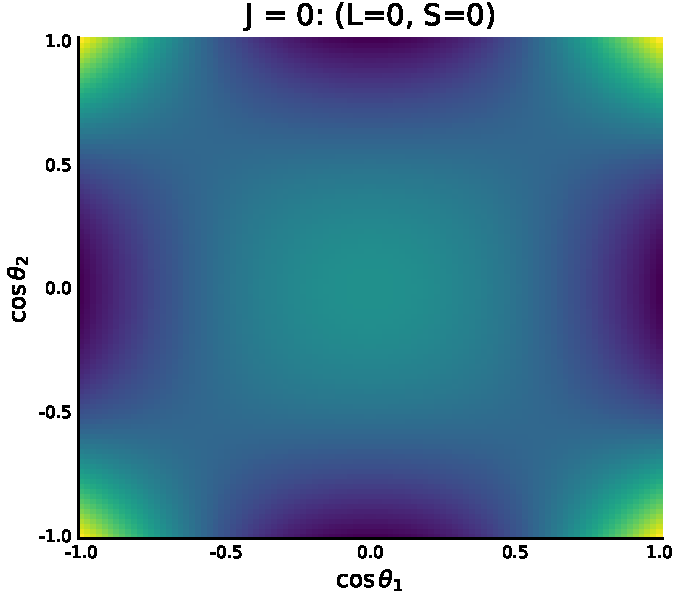
\includegraphics[width=0.195\textwidth]{../plots/map_JLS_000.pdf}
%   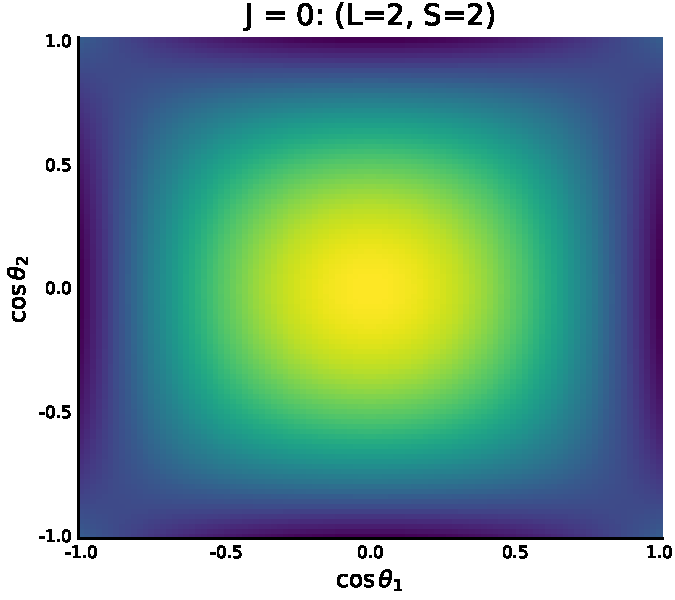
\includegraphics[width=0.195\textwidth]{../plots/map_JLS_022.pdf}
%   \caption{}
%   \label{fig.j0}
% \end{figure}
% \begin{figure}
%   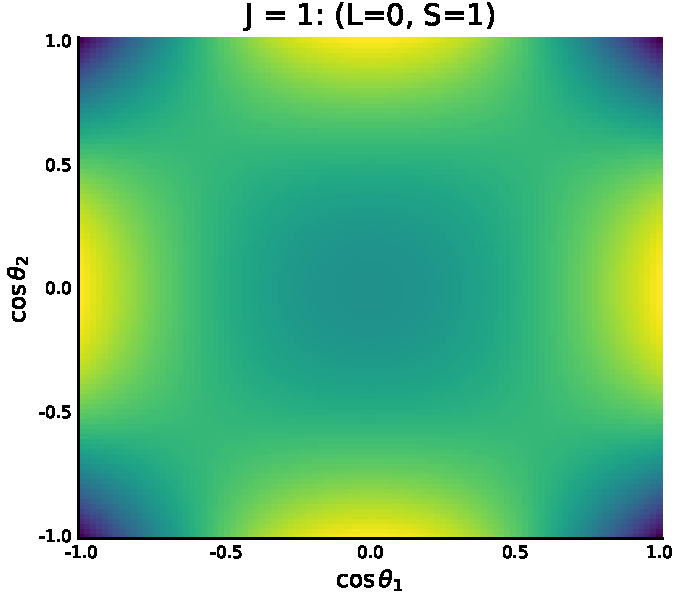
\includegraphics[width=0.195\textwidth]{../plots/map_JLS_101.pdf}
%   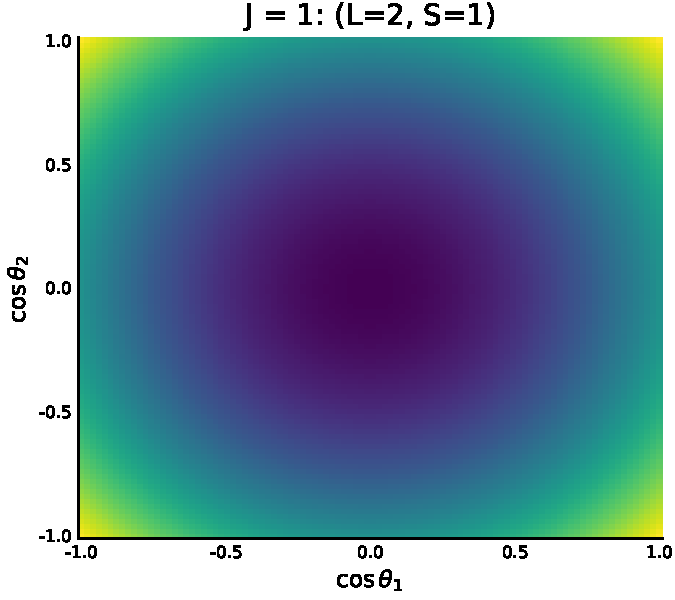
\includegraphics[width=0.195\textwidth]{../plots/map_JLS_121.pdf}
%   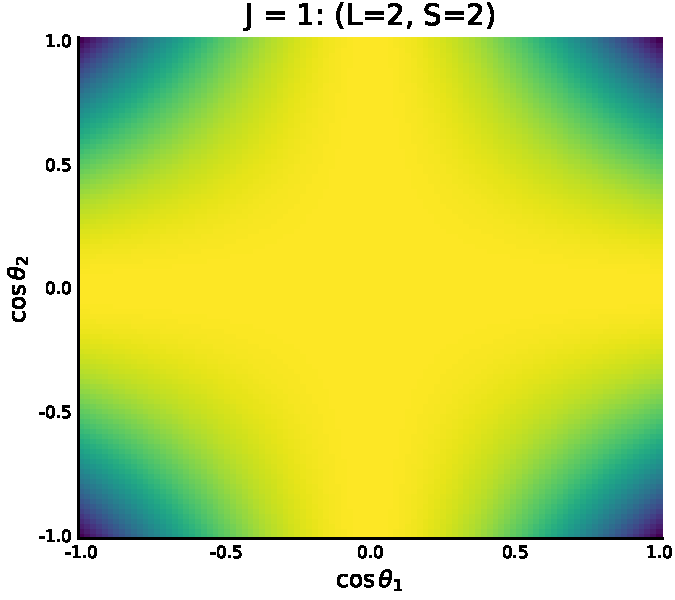
\includegraphics[width=0.195\textwidth]{../plots/map_JLS_122.pdf}
%   \caption{}
%   \label{fig.j1}
% \end{figure}
% \begin{figure}
%   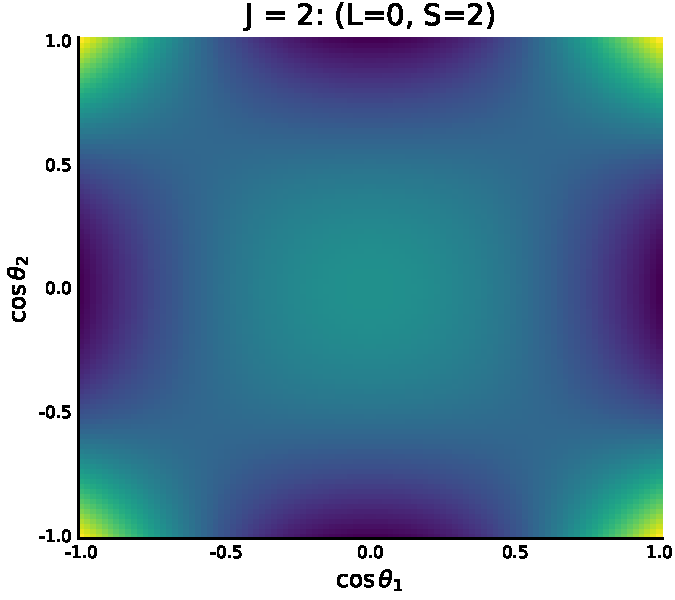
\includegraphics[width=0.195\textwidth]{../plots/map_JLS_202.pdf}
%   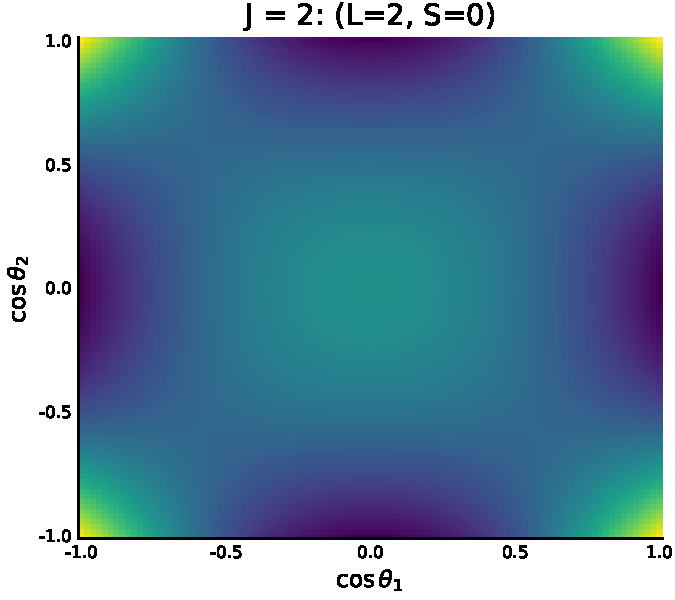
\includegraphics[width=0.195\textwidth]{../plots/map_JLS_220.pdf}
%   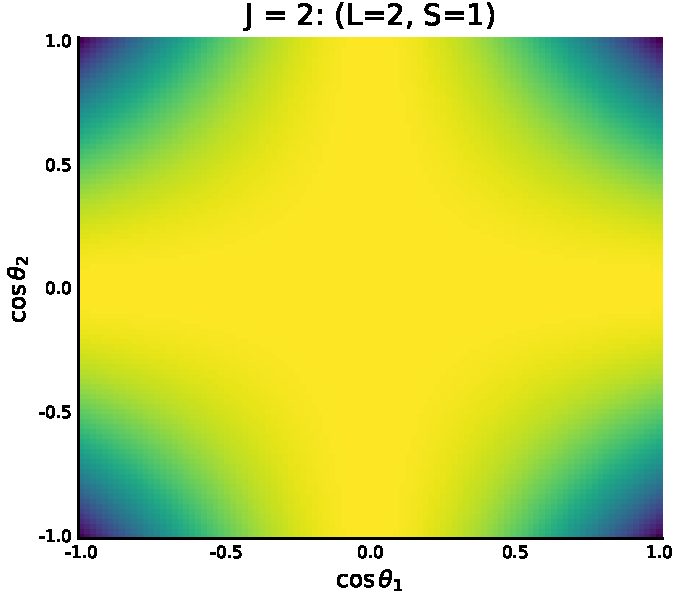
\includegraphics[width=0.195\textwidth]{../plots/map_JLS_221.pdf}
%   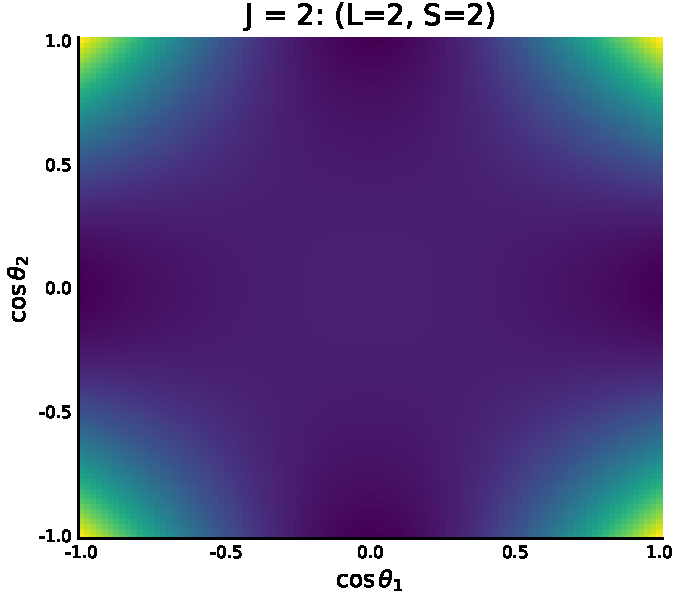
\includegraphics[width=0.195\textwidth]{../plots/map_JLS_222.pdf}
%   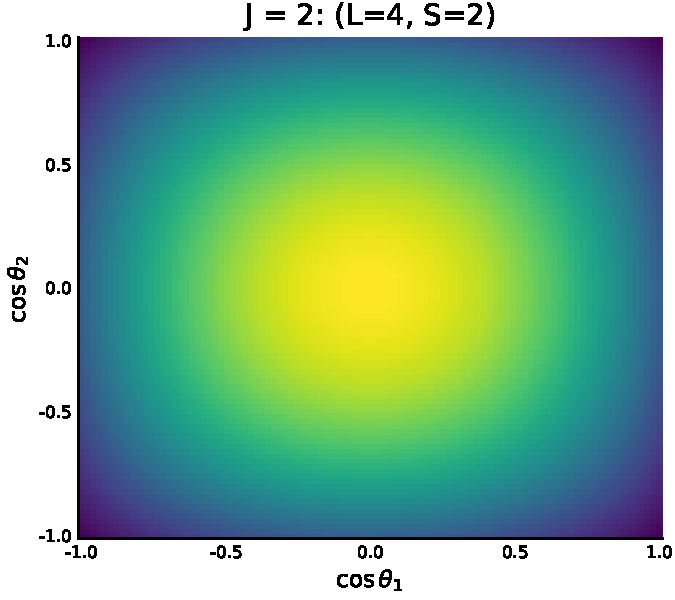
\includegraphics[width=0.195\textwidth]{../plots/map_JLS_242.pdf}
%   \caption{}
%   \label{fig.j2}
% \end{figure}


% \begin{align}
%     I(\cos\theta_1,\phi_1,\cos\theta_2,\phi_2) &= 9\sum_{M}P_M
%     \sum_{\lambda_1,\lambda_2}\sum_{\lambda_1',\lambda_2'}
%     d_{M,\lambda_1-\lambda_2}^{J}(\theta) (-1)^{1-\lambda_2}
%     d_{M,\lambda_1'-\lambda_2'}^{J}(\theta) (-1)^{1-\lambda_2'}
%     \\ \nonumber
%     &\qquad\times
%     H_{\lambda_1\lambda_2} H_{\lambda_1'\lambda_2'}^{*}
%     e^{i(\lambda_1'-\lambda_1)\phi_1}
%     e^{i(\lambda_2'-\lambda_2)\phi_2}
%     \\ \nonumber
%     &\qquad\times
%     \sum_{\xi_1}^{\{-1,1\}}
%     d_{\lambda_1,\xi_1}^{1}(\theta_1) d_{\lambda_1',\xi_1}^{1}(\theta_1)
%     \sum_{\xi_2}^{\{-1,1\}}
%     d_{\lambda_2,\xi_2}^{1}(\theta_2) d_{\lambda_2',\xi_2}^{1}(\theta_2).
% \end{align}
